



\documentclass{beamer}
\usepackage[utf8]{inputenc}
\usepackage{url}
\usepackage{algorithm}
\usepackage{algpseudocode}
\usepackage{lmodern}
\usepackage{natbib}
\usepackage{tikz}
\usepackage{physics}
\usepackage{graphicx} % Allows including images
\graphicspath{ {./images/} }
\usepackage{booktabs} % Allows the use of \toprule, \midrule and \bottomrule in tables
\usepackage{tikz}
\usetikzlibrary{arrows.meta}

\usetikzlibrary{mindmap, trees, shadows, shapes, calc, fadings, positioning, decorations.pathreplacing, intersections, shapes, arrows}

%\usetheme{Hannover}
%\usecolortheme{spruce}
% EPIC FAIL
\usetheme{default}
%\usecolortheme{beetle}
\usepackage{graphics}

\usepackage{color}
\definecolor{new_turquoise}{RGB}{40,151,158}%{251,190,94}
\setbeamercolor{title}{fg=new_turquoise}


%\usepackage[colorlinks=true, urlcolor=blue, linkcolor=red]{hyperref}


\makeatletter
\setbeamertemplate{frametitle}{
    \ifbeamercolorempty[bg]{frametitle}{}{\nointerlineskip}%
    \@tempdima=\textwidth%
    \advance\@tempdima by\beamer@leftmargin%
    \advance\@tempdima by\beamer@rightmargin%
    \vspace*{0.8cm} 
    %\hspace*{-3cm}
    %%%%%%%%%%%%% For example insert shift to right
    \begin{beamercolorbox}[sep=0.3cm,center,wd=\the\@tempdima]{frametitle}
        \usebeamerfont{frametitle}%
        \vbox{}\vskip-1ex%
        \if@tempswa\else\csname beamer@ftecenter\endcsname\fi%
        \strut\insertframetitle\strut\par%
        {%
            \ifx\insertframesubtitle\@empty%
            \else%
            {\usebeamerfont{framesubtitle}\usebeamercolor[fg]{framesubtitle}\insertframesubtitle\strut\par}%
            \fi
        }%
        \vskip-1ex%
        \if@tempswa\else\vskip-.3cm\fi% set inside beamercolorbox... evil here...
    \end{beamercolorbox}%
}
\makeatother

\setbeamercolor{frametitle}{fg=new_turquoise}
\setbeamertemplate{itemize item}{\color{new_turquoise}$\blacksquare$}
\setbeamertemplate{itemize subitem}{\color{new_turquoise}$\blacksquare$}


% --- ENUMERATE ITEMS ---
\setbeamertemplate{enumerate item}{\color{new_turquoise}\insertenumlabel}
\setbeamertemplate{enumerate subitem}{\color{new_turquoise}\insertsubenumlabel}

\setbeamertemplate{caption}{\raggedright\insertcaption\par}

% --- COLOR THE TABLE OF CONTENTS ENTRIES ---
\setbeamercolor{section in toc}{fg=new_turquoise}
\setbeamercolor{subsection in toc}{fg=new_turquoise}
\setbeamercolor{subsubsection in toc}{fg=new_turquoise}



\usebackgroundtemplate{
    
\includegraphics[width=\paperwidth,height=\paperheight]{figs/slide-title.jpg}
} 

\title{\fontsize{49}{7.2}{\bf Fundamental Algorithmic Techniques IX}}
%\author{JW}
\date{\color{new_turquoise}\today}
%S\titlegraphic{\includegraphics[width=2cm]{figs/jw.png}}

\begin{document}
\frame{\titlepage}
%% SLIDE 1 - INTRO TO THE TEAM
%%%%%%%%%%%%%%%%%%%%%%%%%%%%%%%%%%%%%%%%%%%%%%%%%%%%%

\usebackgroundtemplate{
    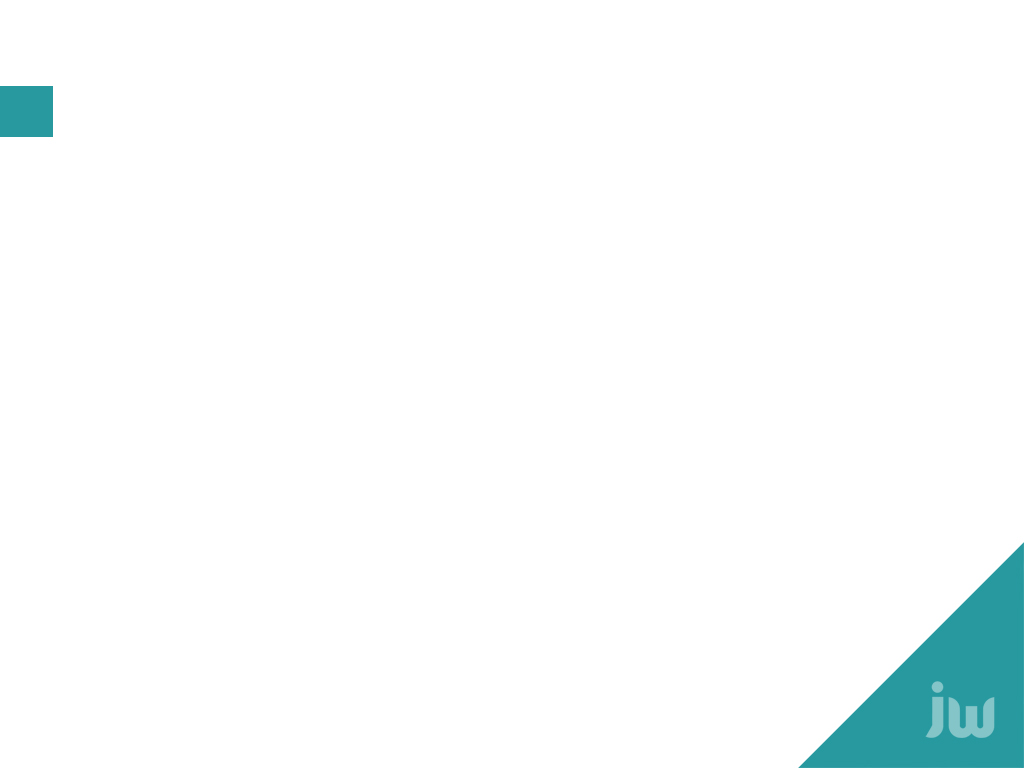
\includegraphics[width=\paperwidth,height=\paperheight]{figs/slide-pages}
} 


\setbeamertemplate{subsection in toc}{
  \color{new_turquoise}$\blacksquare$\color{black}~~\inserttocsubsection
}


% Outline frame
\begin{frame}{Outline}
    \tableofcontents
\end{frame}



\section{Topological Sort}



\begin{frame}{Topological Sort: DFS Approach}

\begin{columns}[T]

% ============= LEFT COLUMN =============
\begin{column}{0.55\textwidth}
    %\vspace{0.5cm}
    %\Large\textbf{Key Points}
    \tiny

    \vspace{0.4cm}
    \begin{itemize}
        \item Works only on \textbf{Directed Acyclic Graphs} (DAGs)
        \item Detects cycles (if any node is visited twice)
        \item Result is \textbf{not unique} in general
        \item All trees have a topological order
        \item 
 Course prerequisites, Build/makefile dependencies, Class loading in Java
    \end{itemize}

    \vspace{0.4cm}
    \centering
    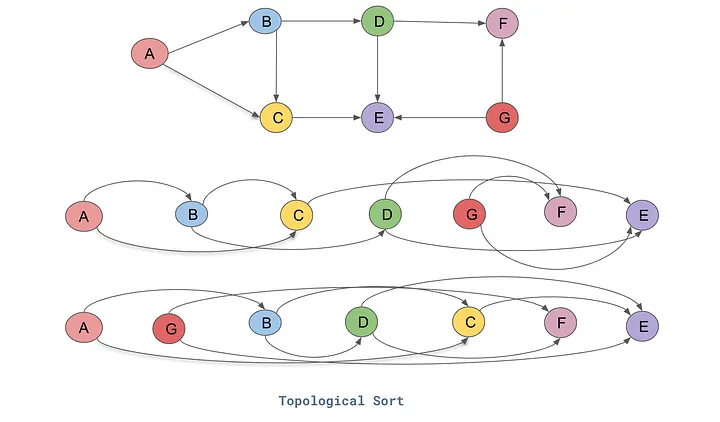
\includegraphics[height=4.2cm]{Algos_figs/topsort.png}  
    
\end{column}

% ============= RIGHT COLUMN =============
\begin{column}{0.45\textwidth}
    %\textbf{DFS-based Algorithm} \quad $O(V+E)$
    %\vspace{0.3cm}

\textcolor{new_turquoise}{Algorithm}:\\
Create empty stack $S_{topo}$
\begin{enumerate}
    \item pick random starting node
    \item run DPS until node has no children (cancel edges along the way)
    \item push childrenless node into $S_{topo}$
    \item perform DPS further if possible, if not start from new node.
\end{enumerate}


\end{column}

\end{columns}
\end{frame}




\section{Cycles Detection}


\begin{frame}{Cycle Detection: DFS vs BFS — Complexity}
  \begin{center}
    % Place two images side by side
    \begin{minipage}{0.48\textwidth}
      \centering
      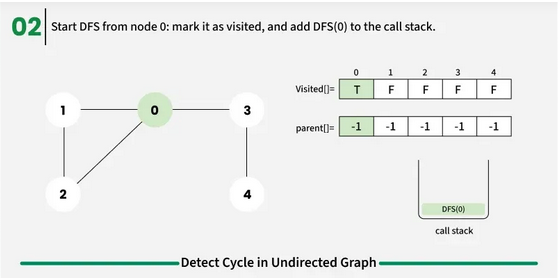
\includegraphics[width=\textwidth]{Algos_figs/depthfirst_clique_1.png} \\
      \small Depth-First Search step 0
    \end{minipage}
    \hfill
    \begin{minipage}{0.48\textwidth}
      \centering
      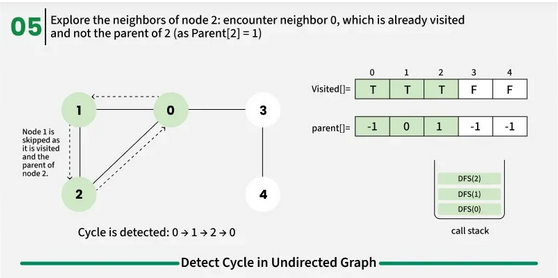
\includegraphics[width=\textwidth]{Algos_figs/depthfirst_clique_2.png} \\
      \small Depth-First Search step 3
    \end{minipage}
  \end{center}

\tiny
  \vspace{1em}
  \textbf{Both detect the cycle} when exploring the back edge (e.g., $D \rightarrow A$): \\
  since the target node is already visited and not the immediate parent (in undirected) or is on the recursion stack (in directed).

  \vspace{1em}
  \textbf{Complexity:}
  \begin{itemize}
  \item \textbf{Time: $O(V + E)$} for both \\
          Every vertex and edge is processed at most once.
    \item \textbf{Space: $O(V)$} for both \\
          \begin{itemize}
            \item \textbf{DFS}: Call stack depth ≤ $V$ (worst-case path).
            \item \textbf{BFS}: Queue may hold up to $O(V)$ nodes (e.g., wide level).
  \end{itemize}
  \end{itemize}

\end{frame}



\begin{frame}{Bron–Kerbosch Algorithm: \\Maximal Clique Enumeration}
\begin{columns}
\begin{column}{0.55\textwidth}
\footnotesize
Undirected graph $G = (V, E)$, \\$N(v)$ = neighbors of $v$ in $G$,\\
\vspace{0.4em}

\vspace{0.6em}
\textbf{Initial call:} \texttt{BronKerbosch1($\emptyset$, $V$, $\emptyset$)}

\vspace{0.6em}
\textbf{Pseudocode:}
\par\nobreak{\footnotesize
\texttt{algorithm BronKerbosch1(R, P, X) is}\\
\texttt{~~~~if P and X are both empty then}\\
\texttt{~~~~~~~~report R as a maximal clique}\\
\texttt{~~~~for each vertex v in P do}\\
\texttt{~~~~~~~~BronKerbosch1(R $\cup$ \{v\}, P $\cap$ N(v), X $\cap$ N(v))}\\
\texttt{~~~~~~~~P := P $\setminus$ \{v\}}\\
\texttt{~~~~~~~~X := X $\cup$ \{v\}}\\
}
\end{column}

\begin{column}{0.45\textwidth}
\vspace{1em}
\begin{center}
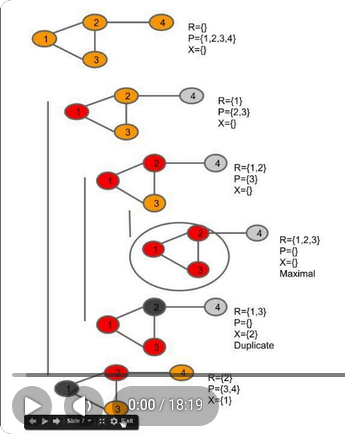
\includegraphics[width=\textwidth]{Algos_figs/Bron–Kerbosch Algorithm-YouTube.png} % Replace with your image
\end{center}
\end{column}
\end{columns}
\end{frame}




\section{Connected Components}






\begin{frame}
\frametitle{Kosaraju's Algorithm - Strongly Connected Components}
\begin{columns}
\begin{column}{0.55\textwidth}
\begin{block}{\textcolor{new_turquoise} {Kosaraju's Algorithm}} %jair
\small
\begin{enumerate}
    \item \textbf{DFS on Original Graph}: Record finish times
    \item \textbf{Transpose the Graph}: Reverse all edges
    \item \textbf{DFS on Transposed Graph}: Process nodes in order of decreasing finish times to find SCCs
\end{enumerate}
\end{block}

\vspace{0.5em}
\begin{itemize}

\item \textbf{Time Complexity}: Depth First Search: $\mathcal{O}(V + E)$
    \item \textbf{Space Complexity}: Stack: $\mathcal{O}(V)$
    %\item \textbf{Key Insight}: The transpose preserves SCCs but reverses the direction between components — enabling sequential discovery
\end{itemize}
\end{column}

\begin{column}{0.45\textwidth}
\begin{center}
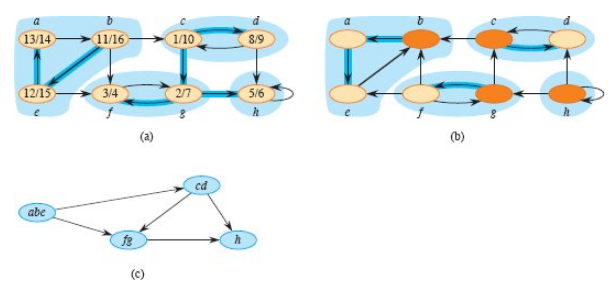
\includegraphics[width=0.5\textheight]{Algos_figs/Kosaraju.png}
\\[1em]
\small Two-pass DFS to find SCCs
\end{center}
\end{column}
\end{columns}
\end{frame}









\begin{frame}{Tarjan's Algorithm for SCCs}

\begin{columns}[T]
    \column{0.48\textwidth}
    \centering
    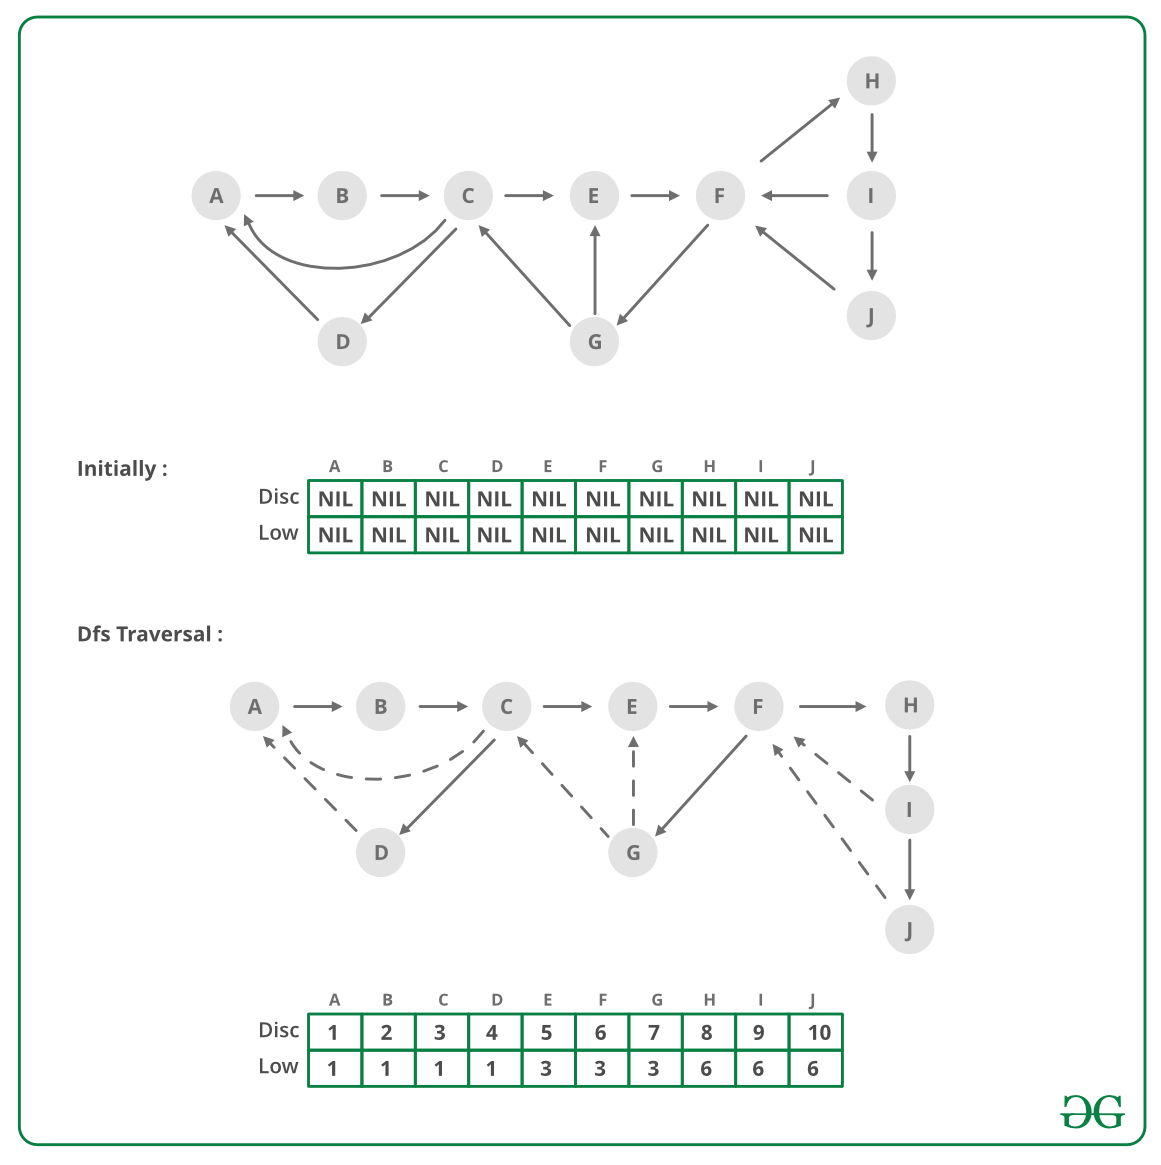
\includegraphics[width=\textwidth]{Algos_figs/TarjansAlgorithms.png}

    \column{0.48\textwidth}
    \textcolor{new_turquoise}{\bf Index}: Discovery order in DFS\\
    \textcolor{new_turquoise}{\bf Low-link}: Smallest index reachable via DFS (including back edges)\\[0.2cm]
    
    \textbf{Problem}: Random DFS order → ambiguous SCC boundaries\\[0.2cm]
    
    \textbf{Solution}: Use a stack to track active nodes\\
    \textbullet\ When $\texttt{low}[u] = \texttt{index}[u]$: pop stack until $u$ — those form one SCC\\[0.2cm]
    
    \textcolor{new_turquoise}{\bf Complexity}: $\mathcal{O}(V + E)$   \\node/edge visited once
\end{columns}

\end{frame}



\section{Minimum Spanning Trees}




\begin{frame}{Jarník’s (Prim's) Algorithm}
\begin{columns}
\begin{column}{0.5\textwidth}
\begin{figure}
\centering
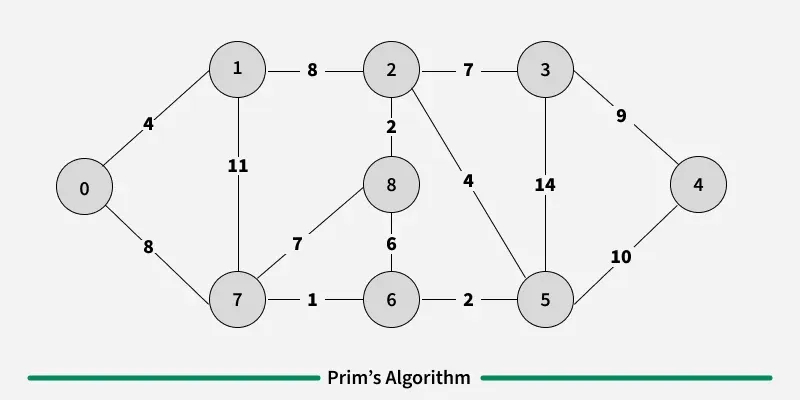
\includegraphics[width=0.9\textwidth]{Algos_figs/Prims-Algorithm-1.png} \\
\vspace{0.2em}
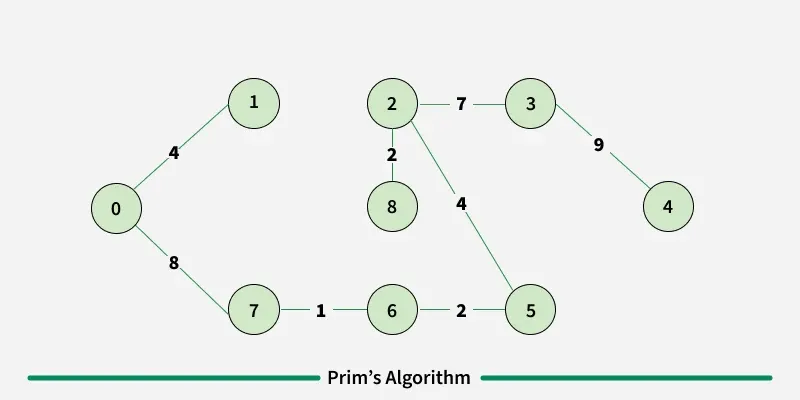
\includegraphics[width=0.9\textwidth]{Algos_figs/Prims-Algorithm-11.png}
\caption{Prim's Algorithm: initial graph (top) and MST }
\end{figure}
\end{column}

\begin{column}{0.5\textwidth}
\footnotesize
\textcolor{new_turquoise}{\bf Steps}
\begin{enumerate}
\item Start from arbitrary vertex for MST.
\item Till there are fringe vertices:
\item Find edges connecting tree \& fringe vertices
\item Find the minimum among these edges
\item Add the chosen edge to the MST
\item Return the MST
\end{enumerate}

\textcolor{new_turquoise}{\bf Complexity}
\begin{itemize}
    \item Time: $\mathcal{O}(E\cdot \mathrm{log} V)$  \\
with binary heap
    \item Space: $\mathcal{O}(V)$
\end{itemize}
\end{column}
\end{columns}
\end{frame}


\begin{frame}{Cuts and the Cut Property}
\textcolor{new_turquoise}{\bf Definition (Cut)}\\
A \emph{cut} $(S, V \setminus S)$ of an undirected graph $G = (V, E)$ is a partition of $V$ into two non-empty disjoint subsets $S$ and $V \setminus S$.

\textcolor{new_turquoise}{\bf Cut-Crossing Edge}\\
An edge $(u,v) \in E$ \emph{crosses} the cut if exactly one of $u$ or $v$ is in $S$.

\textcolor{new_turquoise}{\bf Cut Property / Theorem}\\
For any cut $(S, V \setminus S)$, {\bf if edge $e$'s weight is the minimum among all edges crossing the cut, then $e$ belongs to \emph{some} MST of $G$}.

\vspace{0.3cm}
\begin{columns}[T]
\column{0.5\textwidth}
\centering
\textbf{Cut Illustration}\\
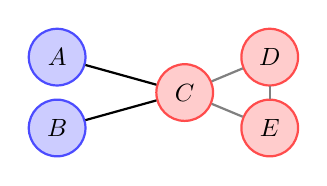
\begin{tikzpicture}[scale=0.9, transform shape]
  % Nodes in S (blue)
  \node[circle, draw=blue!70, fill=blue!20, thick, minimum size=0.8cm] (A) at (0,1) {$A$};
  \node[circle, draw=blue!70, fill=blue!20, thick, minimum size=0.8cm] (B) at (0,0) {$B$};

  % Nodes not in S (red)
  \node[circle, draw=red!70, fill=red!20, thick, minimum size=0.8cm] (C) at (1.8,0.5) {$C$};
  \node[circle, draw=red!70, fill=red!20, thick, minimum size=0.8cm] (D) at (3,1) {$D$};
  \node[circle, draw=red!70, fill=red!20, thick, minimum size=0.8cm] (E) at (3,0) {$E$};

  % Non-crossing edges (gray)
  \draw[gray, thick] (C) -- (D);
  \draw[gray, thick] (C) -- (E);
  \draw[gray, thick] (D) -- (E);

  % Crossing edges (black, solid)
  \draw[black, thick] (A) -- (C);
  \draw[black, thick] (B) -- (C);
\end{tikzpicture}

\column{0.5\textwidth}
\centering
\textbf{Cut Property in Action}\\
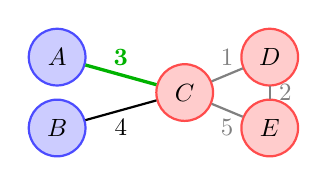
\begin{tikzpicture}[scale=0.9, transform shape]
  % Nodes in S (blue)
  \node[circle, draw=blue!70, fill=blue!20, thick, minimum size=0.8cm] (A) at (0,1) {$A$};
  \node[circle, draw=blue!70, fill=blue!20, thick, minimum size=0.8cm] (B) at (0,0) {$B$};

  % Nodes not in S (red)
  \node[circle, draw=red!70, fill=red!20, thick, minimum size=0.8cm] (C) at (1.8,0.5) {$C$};
  \node[circle, draw=red!70, fill=red!20, thick, minimum size=0.8cm] (D) at (3,1) {$D$};
  \node[circle, draw=red!70, fill=red!20, thick, minimum size=0.8cm] (E) at (3,0) {$E$};

  % Non-crossing edges (gray, with weights)
  \draw[gray, thick] (C) -- (D) node[midway, above] {$1$};
  \draw[gray, thick] (C) -- (E) node[midway, below] {$5$};
  \draw[gray, thick] (D) -- (E) node[midway, right] {$2$};

  % Crossing edges: highlight minimum with green
  \draw[green!70!black, very thick] (A) -- (C) node[midway, above] {$\mathbf{3}$};
  \draw[black, thick] (B) -- (C) node[midway, below] {$4$};
\end{tikzpicture}
\end{columns}

\textcolor{new_turquoise}{\bf Note:} The green edge (weight 3) is the lightest \\ crossing edge and must appear in \emph{some} MST.
\end{frame}






% Slide 2: Proof of Correctness
\begin{frame}{MST Building: Proof of Correctness}
\textcolor{new_turquoise}{\bf Key Invariant}\\
At each step, the tree $T$ maintained by the algorithm is a subset of some MST.


\textcolor{new_turquoise}{\bf Proof by Induction}
\begin{itemize}
\item \textbf{Base Case:} $T = \{v_0\}$ is trivially part of an MST.
\item \textbf{Inductive Step:} Assume $T$ is part of MST $T^*$. Let $e = (u,v)$ be the minimum-weight edge crossing the cut $(T, V \setminus T)$.
\begin{itemize}
\item If $e \in T^*$: $T \cup \{e\}$ still part of $T^*$.
\item If $e \notin T^*$: $\exists e' \in T^*$ crossing same cut. Then $T^* - \{e'\} \cup \{e\}$ is also an MST (by cut property), since $w(e) \leq w(e')$.
\end{itemize}
\end{itemize}

\textcolor{new_turquoise}{\bf Conclusion}\\
By induction, $T$ is always part of an MST. \\ Final $T$ is a spanning tree $\Rightarrow$ it is an MST.
\end{frame}


\begin{frame}{Jarník's Algorithm: Binary Heap Implementation}
\begin{columns}
\begin{column}{0.7\textwidth}
\begin{algorithm}[H]
\tiny
\begin{algorithmic}[1]
\Procedure{JarnikMST}{$G=(V,E)$}
    \State $Q \gets$ empty min-heap \Comment{Vertices with key values}
    %\State $parent[v] \gets \text{null}$ 
    \For{$v \in V$}
        \State $key[v] \gets \infty$
        \State $Q$.insert($v, key[v]$)
    \EndFor
    \State $key[0] \gets 0$ \Comment{Start from vertex 0}
    \While{$Q$ is not empty}
        \State $u \gets Q$.extractMin()
        \For{$v \in$ Adj[$u$] \textbf{and} $v \in Q$}
            \If{$w(u,v) < key[v]$}
                \State $parent[v] \gets u$
                \State $key[v] \gets w(u,v)$
            \EndIf
        \EndFor
    \EndWhile
\EndProcedure
\end{algorithmic}
\end{algorithm}
\end{column}
\begin{column}{0.3\textwidth}
\begin{figure}
\centering
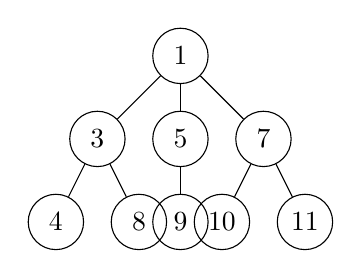
\begin{tikzpicture}[
    node/.style={circle, draw, minimum size=20pt, inner sep=2pt},
    level distance=30pt,
    level 1/.style={sibling distance=30pt}
]

% Root node
\node[node] (root) {1}
    % Level 1 children (3 neighbors)
    child { node[node] (left) {3}
        child { node[node] (leftleft) {4} }
        child { node[node] (leftright) {8} }
    }
    child { node[node] (middle) {5}
        child { node[node] (middleleft) {9} }
    }
    child { node[node] (right) {7}
        child { node[node] (rightleft) {10} }
        child { node[node] (rightright) {11} }
    };



\end{tikzpicture}
\caption{Min-heap example with 3 children for root}
\end{figure}
\end{column}
\end{columns}

\textbf{Complexity:} $O(E \log V)$ if using min heap \\(Faster alternative with Fibonacci)
\end{frame}





\begin{frame}
\frametitle{Kruskal's Algorithm - Greedy MST Construction}

\textcolor{new_turquoise}{\bf Kruskal's Algorithm Steps}
\begin{enumerate}
    \item \textbf{Initialize DSU}: Each vertex in its own component
    \item \textbf{Sort edges}: By weight (ascending order)
    \item \textbf{For each edge} $(u,v)$ in sorted order:
    \item \textbf{Check for cycle}: If \texttt{find(u)} $\neq$ \texttt{find(v)}
        \item \textbf{Add to MST}: Include edge if no cycle
        \item \textbf{Union}: Merge components using \texttt{union(u,v)}
        \item \textbf{Skip}: If same component (cycle detected)
\end{enumerate}

\vspace{1em}
\textcolor{magenta}{\bf Greedy Strategy} \\
Always pick the smallest available edge that doesn't create a cycle

\end{frame}


\begin{frame}{Kruskal Algorithm: Execution}
\begin{center}
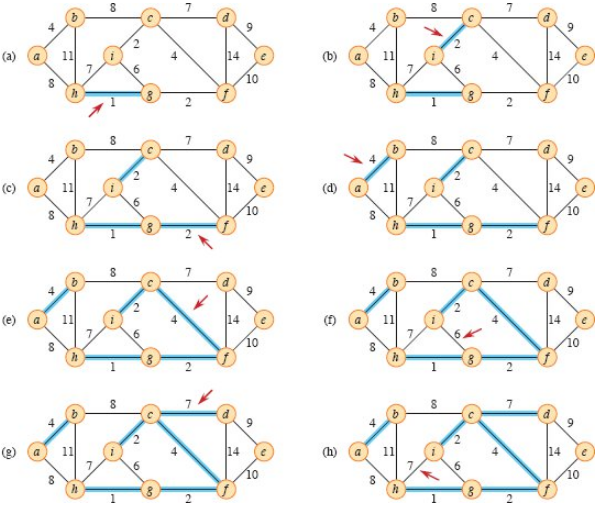
\includegraphics[width=0.7\textwidth]{Algos_figs/kruskal_execution.png}
\end{center}
\begin{center}
\footnotesize\textit{Stepwise execution of Kruskal Algorithm}
\end{center}
\end{frame}














\end{document}


